\scanpage{31}\mspage{30}
% @ top, part a
a) $F'$ est une figure. \deleted{i.e.} Notons que \deleted{$|F'|=$}
% @ top, support with braces
\[
 |F'|=\underbrace{|G'|}_{|G|}\cup\underbrace{|F\setminus G|}_{\supset |F|\setminus |G|}\deleted{\unsure{=|\supset}}\supset |F|
\]
% @ upper part, connector
donc, comme $|F'|\subset |F|$, on a
% @ upper part, support equality
\[
 |F'|\unsure{=|\supseteq|\geq}|F|
\]
% @ upper part, argument
Il faut prouver que $\forall x\in |F'|=|F|$, $\exists$ plus petit \unsure{élémt|élément|élt} de $F'$ qui le contienne. Distinguons deux cas

% @ upper middle, first case
1$^\circ$) $x\in |G|=|G'|$, soit $A\in \unsure{{G'}^\bullet|{G'}^{\deleted{\circ}}}$ tel que $x\in A^{\circ(G')\deleted{\unsure{)|?}}}$. Si $B\in F'$ et \deleted{$B\unsure{\ni|\supset}$} $x\in B$, prouvons $A\subset B$. Si $B\in G'$, c'est évident. Si $B\in F\setminus G$, alors \deleted{$B$ contient} $A^{\circ(G')}\cap B\ne\varnothing$ donc $A^{\unsure{\bullet|\circ}}\subset B$ OK

% @ middle, second case
2$^\circ$) $x\in |\deleted{\unsure{G}}F|\setminus |G|$, alors les $\deleted{B}A\in F'$ qui contiennent $x$ ne sont pas dans $G'$, ils sont donc dans $F\setminus G$. D'autre part, l'unique \unsure{élémt|élément|élt} $A$ de $F$ tel que $x\in A^{\circ(F)}$ n'est pas dans $G$ puisque $x\notin |G|$, il est donc dans $F\setminus G$, et \deleted{\unsure{si $x\in A$}} c'est lui plus petit él. de $F$ (et à fortiori de $F\setminus G$) qui contient $x$, OK~!

% @ lower middle, part b
b) $F'$ \deleted{raffine}\inserted{subdivise} $F$. Comme $|F'|\unsure{=|\supseteq|\geq}|F|$, il faut voir seult que $F'$ raffine $F$. Donc \deleted{que \unsure{tout}} que
% @ lower part, cancelled attempt: interlinear family, original sentence,
% left insertion and lower cancellation enclosure reproduced together
\figure{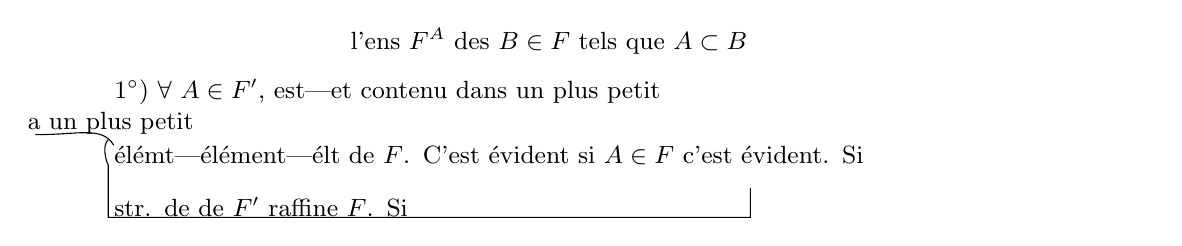
\begin{tikzpicture}[font=\small]
\node[anchor=north west,inner sep=0pt,text width=10.2cm] (family) at (3.0,0.65) {\deleted{\inserted{l'ens $F^A$ des $B\in F$ tels que $A\subset B$}}};
\node[anchor=north west,inner sep=0pt,text width=13.2cm] (attempt) at (0,0) {\deleted{1$^\circ$) \deleted{$\forall$} $A\in F'$, \unsure{est|et} \unsure{contenu dans} un plus petit}};
\node[anchor=north west,inner sep=0pt,text width=13.2cm] (resumption) at (0,-0.85) {\deleted{\unsure{élémt|élément|élt} de $F$. C'est évident si $A\in F$ c'est évident. Si}};
\node[anchor=north west,inner sep=0pt,text width=3.7cm] (addition) at (-1.1,-0.42) {\deleted{\inserted{\unsure{a un plus petit}}}};
\draw ([xshift=3pt]addition.south west) .. controls (-0.45,-0.72) and (-0.15,-0.6) .. (resumption.north west);
\node[anchor=north west,inner sep=0pt,text width=8cm] (abandoned) at (0,-1.5) {\deleted{\unsure{str.} de de $F'$ raffine $F$. Si}};
\draw ([xshift=-2pt,yshift=2pt]resumption.north west)
 .. controls (-0.15,-0.85) and (-0.10,-1.05) .. ([xshift=-2pt]resumption.south west)
 -- ([xshift=-2pt]abandoned.south west)
 -- ([xshift=2pt]abandoned.south east)
 -- ([xshift=2pt,yshift=3pt]abandoned.north east);
\end{tikzpicture}}

% @ lower part, restated first condition
1$^\circ$) \deleted{$\forall$} $A\in F'$, l'ens $F^A=\{B\in F\mid \deleted{B}A\subset B\}$ a un plus petit \unsure{élémt|élément|élt}. C'est évident si $A\in F$ \deleted{$(B=A)$} (on prend $B=A$) et si $A\in G'$, c'est vrai puisque $G'\ll F$.

% @ bottom, second condition
2$^\circ$) Si $A\in F'$, $B\in F$, alors $A\cap B$ est \deleted{\unsure{$\mathcal R_{F'}$-satu.|$\mathscr R_{F'}$-satu.}}\inserted{fermé dans $F'$}
% @ far right edge, beside the final replacement: two unlabelled curved pen strokes
\margin{\figure{\begin{tikzpicture}[x=1ex,y=1ex]
\draw (0,0.45) .. controls (0.25,0.95) and (0.9,1.1) .. (1,0.65)
 .. controls (0.82,0.15) and (0.30,0.12) .. (0.08,0.05);
\draw (0.25,0.45) .. controls (0.5,0.72) and (0.45,0.93) .. (0.7,0.98);
\end{tikzpicture}}}
, i.e. réunion de strates de $F'$. Si $A\in G'$, comme $G'\ll F$, $A\cap B$ est réunion de strates de $G'$, qui sont aussi des strates de $F'$.
